\chapter{Map merging}
\label{sec:mapmerging}
In this chapter the proposed map merging approach is explained. Firstly, the reader will be introduced to the terms needed to explain map merging in general and the new map merging approach especially. Then the previous map merging approach is introduced followed by the new proposed approach.

\section{Terms}

\subsection{\acf{MP} / Landmarks}
The terms \acf{MP} and Landmarks are used interchangeably in this report and are defined as uniquely identifiable objects in the world whose location can be estimated by a sensor \cite{wiki:landmark}.

\subsection{\acf{KF}}
\acfp{KF} are the most representative poses of the trajectory of a robot. As an example in the sketch in figure \autoref{fig:kf}, $x_0$ and $x_3$ are \acp{KF} whereas $x_1$ and $x_2$ are not \acp{KF} as they are not enough representative because they do not contribute additional (unseen) \acp{MP}.

\begin{figure}[H]
   \centering
   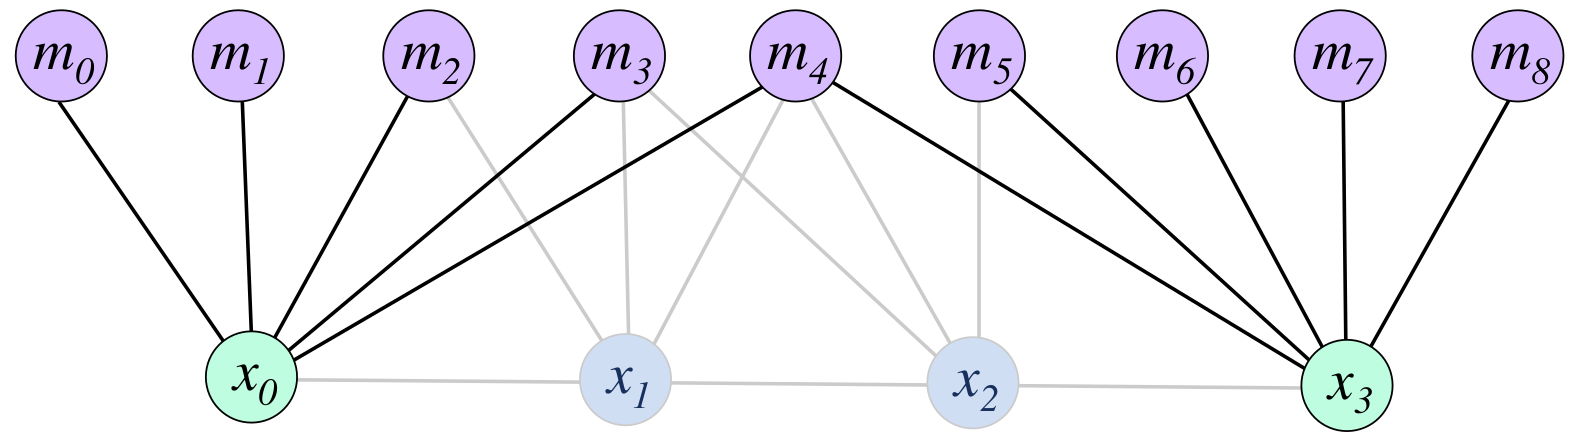
\includegraphics[width=0.75\textwidth]{images/keyframes}
   \caption{Sketch of the \ac{KF} principle}
   \label{fig:kf}
\end{figure}

In ORB-SLAM \cite{Mur-Artal2015}, on which this semester project is based, the following conditions must be fulfilled to insert a new \ac{KF}:

\begin{itemize}
  \item More than 20 frames must have passed from the last global relocalization
  \item Local mapping is idle, or more than 20 frames have passed from last \ac{KF} insertion
  \item Current frame tracks at least 50 points
  \item Current frame tracks less than 90\% points than the reference \ac{KF}
\end{itemize}

\subsection{\acf{KFM}}
A \acf{KFM} is if two \acp{KF}, on per client, observed the same location (\autoref{fig:kfm1}). If a \ac{KFM} was detected a transformation $T \in \text{Sim(3)}$ can be obtained, from the poses of the \acp{KF}, which relates the maps of the two clients to each other (\autoref{fig:kfm2}). With the transformation $T$ the maps than can be aligned (\autoref{fig:kfm3}).

\begin{figure}[H]
  \centering
  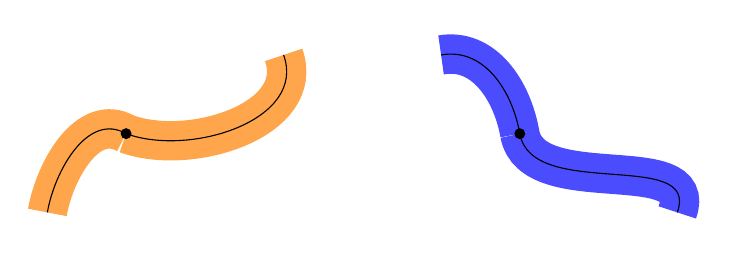
\begin{tikzpicture}
    \coordinate (A) at (0, 0);
    \coordinate (B) at (3, 2);
    \coordinate (C) at (5, 2);
    \coordinate (D1) at (1, 1);
    \coordinate (D2) at (6, 1);
    \coordinate (E) at (8, 0);

    \coordinate (F) at (0.9, 0.9);
    \coordinate (G) at (0.8, 1.1);
    \coordinate (H) at (1.1, 1.1);

    \node at (A) {};
    \node at (B) {};
    \node at (C) {};
    \node at (E) {};

    \draw [orange!70, line width=0.5cm] (A) to [out=80, in=150] (D1);
    \draw [orange!70, line width=0.5cm] (D1) to [out=-20, in=-70] (B);
    \draw [blue!70, line width=0.5cm] (C) to [out=10, in=100] (D2);
    \draw [blue!70, line width=0.5cm] (D2) to [out=-80, in=70] (E);
    \draw [black] (A) to [out=80, in=150] (D1);
    \draw [black] (D1) to [out=-20, in=-70] (B);
    \draw [black] (C) to [out=10, in=100] (D2);
    \draw [black] (D2) to [out=-80, in=70] (E);

    \node [fill=black, circle,inner sep=1pt, text width=0.5mm] at (D1) {};
    \node [fill=black, circle,inner sep=1pt, text width=0.5mm] at (D2) {};
  \end{tikzpicture}
  \caption{Two clients each with own landmarks and \acp{KF} with a \ac{KF} observing the same location}
  \label{fig:kfm1}
\end{figure}

\begin{figure}[H]
  \centering
  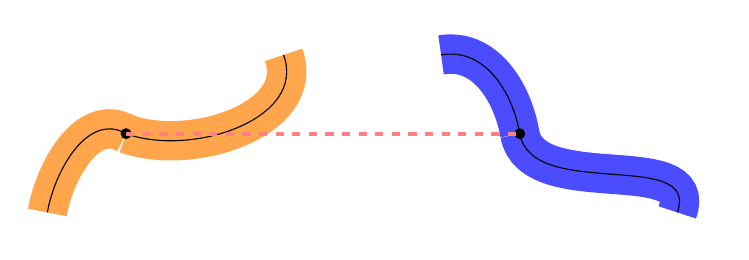
\begin{tikzpicture}
    \coordinate (A) at (0, 0);
    \coordinate (B) at (3, 2);
    \coordinate (C) at (5, 2);
    \coordinate (D1) at (1, 1);
    \coordinate (D2) at (6, 1);
    \coordinate (E) at (8, 0);

    \coordinate (F) at (0.9, 0.9);
    \coordinate (G) at (0.8, 1.1);
    \coordinate (H) at (1.1, 1.1);

    \node at (A) {};
    \node at (B) {};
    \node at (C) {};
    \node at (E) {};

    \draw [orange!70, line width=0.5cm] (A) to [out=80, in=150] (D1);
    \draw [orange!70, line width=0.5cm] (D1) to [out=-20, in=-70] (B);
    \draw [blue!70, line width=0.5cm] (C) to [out=10, in=100] (D2);
    \draw [blue!70, line width=0.5cm] (D2) to [out=-80, in=70] (E);
    \draw [black] (A) to [out=80, in=150] (D1);
    \draw [black] (D1) to [out=-20, in=-70] (B);
    \draw [black] (C) to [out=10, in=100] (D2);
    \draw [black] (D2) to [out=-80, in=70] (E);

    \node [fill=black, circle,inner sep=1pt, text width=0.5mm] at (D1) {};
    \node [fill=black, circle,inner sep=1pt, text width=0.5mm] at (D2) {};

    \draw [red!50, line width=0.05cm, dashed] (D1) to (D2);
  \end{tikzpicture}
  \caption{Transformation $T$ obtained from the poses of the two \acp{KF}}
  \label{fig:kfm2}
\end{figure}

\begin{figure}[H]
  \centering
  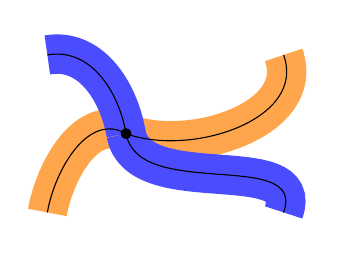
\begin{tikzpicture}
    \coordinate (A) at (0, 0);
    \coordinate (B) at (3, 2);
    \coordinate (C) at (0, 2);
    \coordinate (D) at (1, 1);
    \coordinate (E) at (3, 0);

    \coordinate (F) at (0.9, 0.9);
    \coordinate (G) at (0.8, 1.1);
    \coordinate (H) at (1.1, 1.1);

    \node at (A) {};
    \node at (B) {};
    \node at (C) {};
    \node at (E) {};

    \draw [orange!70, line width=0.5cm] (A) to [out=80, in=150] (D);
    \draw [orange!70, line width=0.5cm] (D) to [out=-20, in=-70] (B);
    \draw [blue!70, line width=0.5cm] (C) to [out=10, in=100] (D);
    \draw [blue!70, line width=0.5cm] (D) to [out=-80, in=70] (E);
    \draw [black] (A) to [out=80, in=150] (D);
    \draw [black] (D) to [out=-20, in=-70] (B);
    \draw [black] (C) to [out=10, in=100] (D);
    \draw [black] (D) to [out=-80, in=70] (E);

    \node [fill=black, circle,inner sep=1pt, text width=0.5mm] at (D) {};
  \end{tikzpicture}
  \caption{The two maps aligned}
  \label{fig:kfm3}
\end{figure}

In conclusion, a \ac{KFM} contains:
\begin{itemize}
  \item Two \acp{KF} (One per map/client)
  \item The transformation ($T \in \text{Sim(3)}$) between the two \acp{KF}
\end{itemize}

\subsection{Co-visibility graph}
Co-visibility is represented as an undirected weighted graph, a co-visibility graph. Each node is a \ac{KF} and an edge between two \acp{KF} exists if they share observations of the same \acp{MP}, being the weight of the edge the number of common \acp{MP} \cite{Mur-Artal2015}. An example of \acp{KF} an the resulting co-visibility graph is shown in \autoref{fig:covis}.

\begin{figure}[H]
	\centering
	\subcaptionbox{\acp{KF} (blue), Current Camera (gree), \acp{MP} (black, red), Current Local \acp{MP} (red)\label{fig:covis1}}{\includegraphics[width=0.45\textwidth]{images/002.eps}}
	\quad
	\subcaptionbox{Co-visibility Graph\label{fig:covis2}}{\includegraphics[width=0.45\textwidth]{images/004.eps}}
	\caption{\acp{KF} and resulting co-visibility graph (Figure taken from \cite{Mur-Artal2015})}
	\label{fig:covis}
\end{figure}

\section{Old approach}
In the old approach, as soon as a \ac{KFM} was detected, the maps were merged. In a real world example this procedure looks the following:

\begin{enumerate}
  \item {Two clients observed the same location (shown in figure \autoref{fig:kfm4})
    \begin{figure}[H]
      \centering
      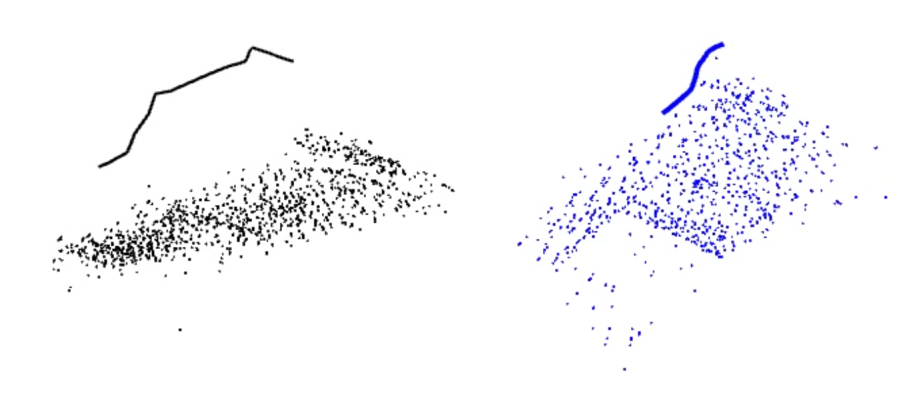
\includegraphics[width=0.75\textwidth]{images/map_1_2_1}
      \caption{Two clients each with own landmarks and \acp{KF} observing the same location}
      \label{fig:kfm4}
    \end{figure}}
  \item {The transformation between the two maps can be obtained (shown in figure \autoref{fig:kfm5})
    \begin{figure}[H]
      \centering
      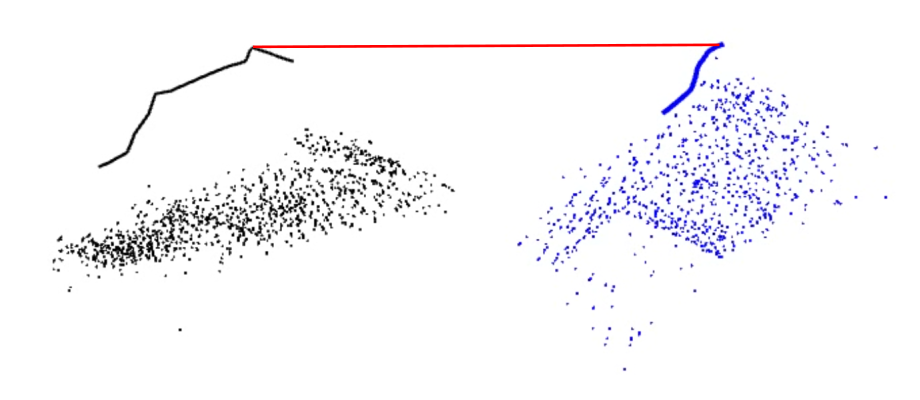
\includegraphics[width=0.75\textwidth]{images/map_1_2_2}
      \caption{Transformation $T$ obtained from the poses of the two \acp{KF}}
      \label{fig:kfm5}
    \end{figure}}
  \item {The maps can be aligned (shown in figure \autoref{fig:kfm6})
    \begin{figure}[H]
      \centering
      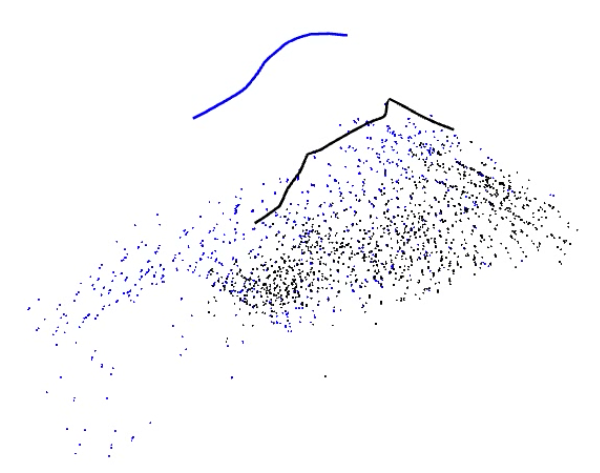
\includegraphics[width=0.75\textwidth]{images/map_1_2_merge}
      \caption{Aligned maps}
      \label{fig:kfm6}
    \end{figure}}
  \item Perform \acf{PGO}
  \item Perform \acf{BA}
\end{enumerate}

\section{New approach}
The proposed map merging approach works as follow:

\begin{enumerate}
  \item After a \ac{KFM} is found skip $m$ \acp{KF} before processing the next \acs{KF}
  \item Wait until $n$ \acp{KFM} were detected
  \item Merge the two maps with the transformation of one of the \acp{KFM}
  \item Fuse map points in the ($n-1$) \acp{KFM}
  \item Perform \ac{PGO}
  \item Perform \ac{BA}
\end{enumerate}

To give the reader a better intuition about how the proposed map merging approach works, it will be visualized in a synthetic example step by step.\\
The example starts with two \acp{KF}, one per client, which are checked if they observe the same location (shown in figure \autoref{fig:newapproach1}). If a \ac{KFM} was detected, as in \autoref{fig:newapproach2}, $m$, in this example five, \acp{KF} are skipped before processing the next \acp{KF} (shown in \autoref{fig:newapproach3}).

\begin{figure}[H]
    \centering
    \subcaptionbox{Two client with one \ac{KF}\label{fig:newapproach1}}{
      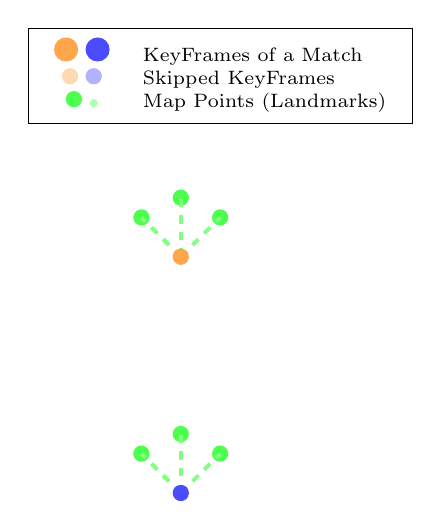
\begin{tikzpicture}
        \coordinate (A1) at (0, 3);
        \coordinate (A1MP1) at (-0.5, 3.5);
        \coordinate (A1MP2) at (0, 3.75);
        \coordinate (A1MP3) at (0.5, 3.5);

        \coordinate (A2) at (0, 0);
        \coordinate (A2MP1) at (-0.5, 0.5);
        \coordinate (A2MP2) at (0, 0.75);
        \coordinate (A2MP3) at (0.5, 0.5);

        \node [fill=green!70, circle,inner sep=2pt, text width=0.1mm] at (A1MP1) {};
        \node [fill=green!70, circle,inner sep=2pt, text width=0.1mm] at (A1MP2) {};
        \node [fill=green!70, circle,inner sep=2pt, text width=0.1mm] at (A1MP3) {};
        \draw [green!50, dashed, line width=0.05cm] (A1) to (A1MP1);
        \draw [green!50, dashed, line width=0.05cm] (A1) to (A1MP2);
        \draw [green!50, dashed, line width=0.05cm] (A1) to (A1MP3);
        \node [fill=orange!70, circle,inner sep=2pt, text width=0.1mm] at (A1) {};

        \node [fill=green!70, circle,inner sep=2pt, text width=0.1mm] at (A2MP1) {};
        \node [fill=green!70, circle,inner sep=2pt, text width=0.1mm] at (A2MP2) {};
        \node [fill=green!70, circle,inner sep=2pt, text width=0.1mm] at (A2MP3) {}; \draw [green!50, dashed, line width=0.05cm] (A2) to (A2MP1);
        \draw [green!50, dashed, line width=0.05cm] (A2) to (A2MP2);
        \draw [green!50, dashed, line width=0.05cm] (A2) to (A2MP3);
        \node [fill=blue!70, circle,inner sep=2pt, text width=0.1mm] at (A2) {};

        \node[draw] at (0.5, 5.3)
        {
          \scriptsize
          \begin{tabular}{cl}
            \tikz\node[fill=orange!70, circle,inner sep=3pt, text width=0.1mm] {}; \tikz\node[fill=blue!70, circle,inner sep=3pt, text width=0.1mm] {}; & KeyFrames of a Match \\
            \tikz\node[fill=orange!30, circle,inner sep=2pt, text width=0.1mm] {}; \tikz\node[fill=blue!30, circle,inner sep=2pt, text width=0.1mm] {}; & Skipped KeyFrames \\
            \tikz\node [fill=green!70, circle, inner sep=2pt, text width=0.1mm] {}; \tikz\node[fill=green!30, circle,inner sep=1pt, text width=0.1mm] {}; & Map Points (Landmarks)
          \end{tabular}
        };
      \end{tikzpicture}}%}
      \quad
    \subcaptionbox{First \ac{KFM}\label{fig:newapproach2}}{
      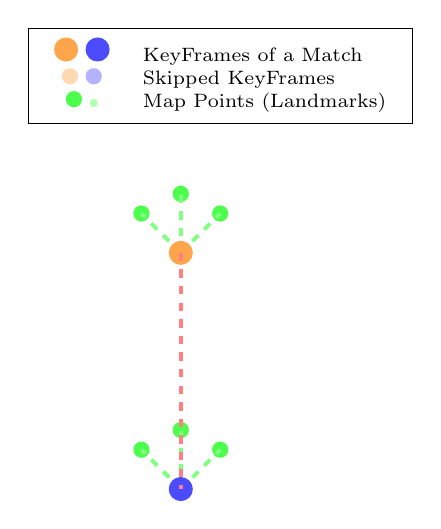
\begin{tikzpicture}
        \coordinate (A1) at (0, 3);
        \coordinate (A1MP1) at (-0.5, 3.5);
        \coordinate (A1MP2) at (0, 3.75);
        \coordinate (A1MP3) at (0.5, 3.5);

        \coordinate (A2) at (0, 0);
        \coordinate (A2MP1) at (-0.5, 0.5);
        \coordinate (A2MP2) at (0, 0.75);
        \coordinate (A2MP3) at (0.5, 0.5);

        \node [fill=green!70, circle,inner sep=2pt, text width=0.1mm] at (A1MP1) {};
        \node [fill=green!70, circle,inner sep=2pt, text width=0.1mm] at (A1MP2) {};
        \node [fill=green!70, circle,inner sep=2pt, text width=0.1mm] at (A1MP3) {};
        \draw [green!50, dashed, line width=0.05cm] (A1) to (A1MP1);
        \draw [green!50, dashed, line width=0.05cm] (A1) to (A1MP2);
        \draw [green!50, dashed, line width=0.05cm] (A1) to (A1MP3);
        \node [fill=orange!70, circle,inner sep=3pt, text width=0.1mm] at (A1) {};

        \node [fill=green!70, circle,inner sep=2pt, text width=0.1mm] at (A2MP1) {};
        \node [fill=green!70, circle,inner sep=2pt, text width=0.1mm] at (A2MP2) {};
        \node [fill=green!70, circle,inner sep=2pt, text width=0.1mm] at (A2MP3) {};
        \draw [green!50, dashed, line width=0.05cm] (A2) to (A2MP1);
        \draw [green!50, dashed, line width=0.05cm] (A2) to (A2MP2);
        \draw [green!50, dashed, line width=0.05cm] (A2) to (A2MP3);
        \node [fill=blue!70, circle,inner sep=3pt, text width=0.1mm] at (A2) {};

        \draw [red!50, line width=0.05cm, dashed] (A1) to (A2);

        \node[draw] at (0.5, 5.25)
        {
          \scriptsize
          \begin{tabular}{cl}
            \tikz\node[fill=orange!70, circle,inner sep=3pt, text width=0.1mm] {}; \tikz\node[fill=blue!70, circle,inner sep=3pt, text width=0.1mm] {}; & KeyFrames of a Match \\
            \tikz\node[fill=orange!30, circle,inner sep=2pt, text width=0.1mm] {}; \tikz\node[fill=blue!30, circle,inner sep=2pt, text width=0.1mm] {}; & Skipped KeyFrames \\
            \tikz\node [fill=green!70, circle, inner sep=2pt, text width=0.1mm] {}; \tikz\node[fill=green!30, circle,inner sep=1pt, text width=0.1mm] {}; & Map Points (Landmarks)
          \end{tabular}
        };
      \end{tikzpicture}}
      \caption{First two steps of the new map merging example}
      \label{fig:newapproach12}
\end{figure}


\begin{figure}[H]
  \centering
  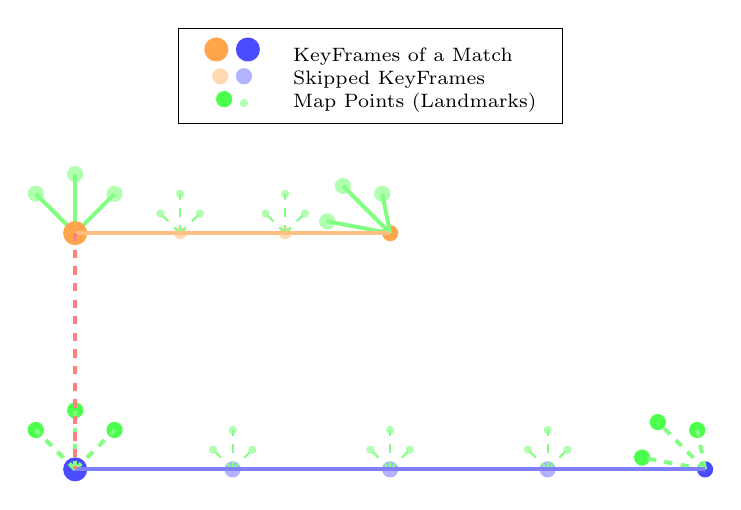
\begin{tikzpicture}
    \coordinate (A1) at (0, 3);
    \coordinate (A1MP1) at (-0.5, 3.5);
    \coordinate (A1MP2) at (0, 3.75);
    \coordinate (A1MP3) at (0.5, 3.5);

    \coordinate (AB11) at (4/3, 3);
    \coordinate (AB11MP1) at (-0.25+4/3, 3.25);
    \coordinate (AB11MP2) at (4/3, 3.5);
    \coordinate (AB11MP3) at (0.25+4/3, 3.25);

    \coordinate (AB12) at (8/3, 3);
    \coordinate (AB12MP1) at (-0.25+8/3, 3.25);
    \coordinate (AB12MP2) at (8/3, 3.5);
    \coordinate (AB12MP3) at (0.25+8/3, 3.25);

    \coordinate (B1) at (4, 3);
    \coordinate (B1MP1) at (3.2, 3.15);
    \coordinate (B1MP2) at (3.4, 3.6);
    \coordinate (B1MP3) at (3.9, 3.5);

    \coordinate (A2) at (0, 0);
    \coordinate (A2MP1) at (-0.5, 0.5);
    \coordinate (A2MP2) at (0, 0.75);
    \coordinate (A2MP3) at (0.5, 0.5);

    \coordinate (AB21) at (2, 0);
    \coordinate (AB21MP1) at (1.75, 0.25);
    \coordinate (AB21MP2) at (2, 0.5);
    \coordinate (AB21MP3) at (2.25, 0.25);

    \coordinate (AB22) at (4, 0);
    \coordinate (AB22MP1) at (3.75, 0.25);
    \coordinate (AB22MP2) at (4, 0.5);
    \coordinate (AB22MP3) at (4.25, 0.25);

    \coordinate (AB23) at (6, 0);
    \coordinate (AB23MP1) at (5.75, 0.25);
    \coordinate (AB23MP2) at (6, 0.5);
    \coordinate (AB23MP3) at (6.25, 0.25);

    \coordinate (B2) at (8, 0);
    \coordinate (B2MP1) at (7.2, 0.15);
    \coordinate (B2MP2) at (7.4, 0.6);
    \coordinate (B2MP3) at (7.9, 0.5);


    \node [fill=green!30, circle,inner sep=2pt, text width=0.1mm] at (A1MP1) {};
    \node [fill=green!30, circle,inner sep=2pt, text width=0.1mm] at (A1MP2) {};
    \node [fill=green!30, circle,inner sep=2pt, text width=0.1mm] at (A1MP3) {};
    \draw [green!50, line width=0.05cm] (A1) to (A1MP1);
    \draw [green!50, line width=0.05cm] (A1) to (A1MP2);
    \draw [green!50, line width=0.05cm] (A1) to (A1MP3);
    \node [fill=orange!70, circle,inner sep=3pt, text width=0.1mm] at (A1) {};

    \node [fill=orange!30, circle,inner sep=1.5pt, text width=0.1mm] at (AB11) {};
    \node [fill=green!30, circle,inner sep=1pt, text width=0.1mm] at (AB11MP1) {};
    \node [fill=green!30, circle,inner sep=1pt, text width=0.1mm] at (AB11MP2) {};
    \node [fill=green!30, circle,inner sep=1pt, text width=0.1mm] at (AB11MP3) {};
    \draw [green!50, dashed, line width=0.025cm] (AB11) to (AB11MP1);
    \draw [green!50, dashed, line width=0.025cm] (AB11) to (AB11MP2);
    \draw [green!50, dashed, line width=0.025cm] (AB11) to (AB11MP3);

    \node [fill=orange!30, circle,inner sep=1.5pt, text width=0.1mm] at (AB12) {};
    \node [fill=green!30, circle,inner sep=1pt, text width=0.1mm] at (AB12MP1) {};
    \node [fill=green!30, circle,inner sep=1pt, text width=0.1mm] at (AB12MP2) {};
    \node [fill=green!30, circle,inner sep=1pt, text width=0.1mm] at (AB12MP3) {};
    \draw [green!50, dashed, line width=0.025cm] (AB12) to (AB12MP1);
    \draw [green!50, dashed, line width=0.025cm] (AB12) to (AB12MP2);
    \draw [green!50, dashed, line width=0.025cm] (AB12) to (AB12MP3);

    \node [fill=orange!70, circle,inner sep=2pt, text width=0.1mm] at (B1) {};
    \node [fill=green!30, circle, inner sep=2pt, text width=0.1mm] at (B1MP1) {};
    \node [fill=green!30, circle, inner sep=2pt, text width=0.1mm] at (B1MP2) {};
    \node [fill=green!30, circle, inner sep=2pt, text width=0.1mm] at (B1MP3) {};
    \draw [green!50, line width=0.05cm] (B1) to (B1MP1);
    \draw [green!50, line width=0.05cm] (B1) to (B1MP2);
    \draw [green!50, line width=0.05cm] (B1) to (B1MP3);

    \node [fill=blue!70, circle,inner sep=3pt, text width=0.1mm] at (A2) {};
    \node [fill=green!70, circle,inner sep=2pt, text width=0.1mm] at (A2MP1) {};
    \node [fill=green!70, circle,inner sep=2pt, text width=0.1mm] at (A2MP2) {};
    \node [fill=green!70, circle,inner sep=2pt, text width=0.1mm] at (A2MP3) {};
    \draw [green!50, dashed, line width=0.05cm] (A2) to (A2MP1);
    \draw [green!50, dashed, line width=0.05cm] (A2) to (A2MP2);
    \draw [green!50, dashed, line width=0.05cm] (A2) to (A2MP3);

    \node [fill=blue!30, circle,inner sep=2pt, text width=0.1mm] at (AB21) {};
    \node [fill=green!30, circle,inner sep=1pt, text width=0.1mm] at (AB21MP1) {};
    \node [fill=green!30, circle,inner sep=1pt, text width=0.1mm] at (AB21MP2) {};
    \node [fill=green!30, circle,inner sep=1pt, text width=0.1mm] at (AB21MP3) {};
    \draw [green!50, dashed, line width=0.025cm] (AB21) to (AB21MP1);
    \draw [green!50, dashed, line width=0.025cm] (AB21) to (AB21MP2);
    \draw [green!50, dashed, line width=0.025cm] (AB21) to (AB21MP3);

    \node [fill=blue!30, circle,inner sep=2pt, text width=0.1mm] at (AB22) {};
    \node [fill=green!30, circle,inner sep=1pt, text width=0.1mm] at (AB22MP1) {};
    \node [fill=green!30, circle,inner sep=1pt, text width=0.1mm] at (AB22MP2) {};
    \node [fill=green!30, circle,inner sep=1pt, text width=0.1mm] at (AB22MP3) {};
    \draw [green!50, dashed, line width=0.025cm] (AB22) to (AB22MP1);
    \draw [green!50, dashed, line width=0.025cm] (AB22) to (AB22MP2);
    \draw [green!50, dashed, line width=0.025cm] (AB22) to (AB22MP3);

    \node [fill=blue!30, circle,inner sep=2pt, text width=0.1mm] at (AB23) {};
    \node [fill=green!30, circle,inner sep=1pt, text width=0.1mm] at (AB23MP1) {};
    \node [fill=green!30, circle,inner sep=1pt, text width=0.1mm] at (AB23MP2) {};
    \node [fill=green!30, circle,inner sep=1pt, text width=0.1mm] at (AB23MP3) {};
    \draw [green!50, dashed, line width=0.025cm] (AB23) to (AB23MP1);
    \draw [green!50, dashed, line width=0.025cm] (AB23) to (AB23MP2);
    \draw [green!50, dashed, line width=0.025cm] (AB23) to (AB23MP3);

    \node [fill=blue!70, circle,inner sep=2pt, text width=0.1mm] at (B2) {};
    \node [fill=green!70, circle,inner sep=2pt, text width=0.1mm] at (B2MP1) {};
    \node [fill=green!70, circle,inner sep=2pt, text width=0.1mm] at (B2MP2) {};
    \node [fill=green!70, circle,inner sep=2pt, text width=0.1mm] at (B2MP3) {};
    \draw [green!50, dashed, line width=0.05cm] (B2) to (B2MP1);
    \draw [green!50, dashed, line width=0.05cm] (B2) to (B2MP2);
    \draw [green!50, dashed, line width=0.05cm] (B2) to (B2MP3);

    \draw [orange!50, line width=0.05cm] (A1) to (B1);
    \draw [blue!50, line width=0.05cm] (A2) to (B2);

    \draw [red!50, line width=0.05cm, dashed] (A1) to (A2);

    \node[draw] at (3.75, 5.0)
    {
      \scriptsize
      \begin{tabular}{cl}
        \tikz\node[fill=orange!70, circle,inner sep=3pt, text width=0.1mm] {}; \tikz\node[fill=blue!70, circle,inner sep=3pt, text width=0.1mm] {}; & KeyFrames of a Match \\
        \tikz\node[fill=orange!30, circle,inner sep=2pt, text width=0.1mm] {}; \tikz\node[fill=blue!30, circle,inner sep=2pt, text width=0.1mm] {}; & Skipped KeyFrames \\
        \tikz\node [fill=green!70, circle, inner sep=2pt, text width=0.1mm] {}; \tikz\node[fill=green!30, circle,inner sep=1pt, text width=0.1mm] {}; & Map Points (Landmarks)
      \end{tabular}
    };
  \end{tikzpicture}
  \caption{Skipped five \acp{KF}}
  \label{fig:newapproach3}
\end{figure}

After $m(= 5)$ \acp{KF} are skipped, the system checks again, if a \ac{KFM} can be detected, shown in \autoref{fig:newapproach3}. \autoref{fig:newapproach4} then shows the case, where the next \ac{KFM} was be detected.

\begin{figure}[H]
  \centering
  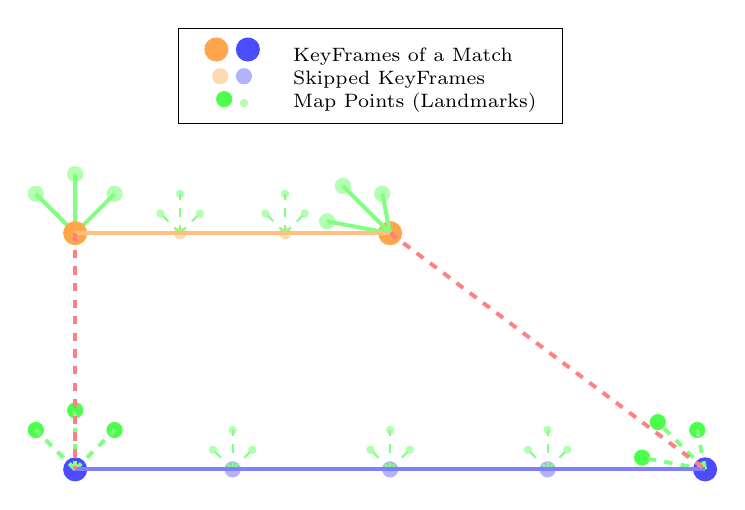
\begin{tikzpicture}
    \coordinate (A1) at (0, 3);
    \coordinate (A1MP1) at (-0.5, 3.5);
    \coordinate (A1MP2) at (0, 3.75);
    \coordinate (A1MP3) at (0.5, 3.5);

    \coordinate (AB11) at (4/3, 3);
    \coordinate (AB11MP1) at (-0.25+4/3, 3.25);
    \coordinate (AB11MP2) at (4/3, 3.5);
    \coordinate (AB11MP3) at (0.25+4/3, 3.25);

    \coordinate (AB12) at (8/3, 3);
    \coordinate (AB12MP1) at (-0.25+8/3, 3.25);
    \coordinate (AB12MP2) at (8/3, 3.5);
    \coordinate (AB12MP3) at (0.25+8/3, 3.25);

    \coordinate (B1) at (4, 3);
    \coordinate (B1MP1) at (3.2, 3.15);
    \coordinate (B1MP2) at (3.4, 3.6);
    \coordinate (B1MP3) at (3.9, 3.5);

    \coordinate (A2) at (0, 0);
    \coordinate (A2MP1) at (-0.5, 0.5);
    \coordinate (A2MP2) at (0, 0.75);
    \coordinate (A2MP3) at (0.5, 0.5);

    \coordinate (AB21) at (2, 0);
    \coordinate (AB21MP1) at (1.75, 0.25);
    \coordinate (AB21MP2) at (2, 0.5);
    \coordinate (AB21MP3) at (2.25, 0.25);

    \coordinate (AB22) at (4, 0);
    \coordinate (AB22MP1) at (3.75, 0.25);
    \coordinate (AB22MP2) at (4, 0.5);
    \coordinate (AB22MP3) at (4.25, 0.25);

    \coordinate (AB23) at (6, 0);
    \coordinate (AB23MP1) at (5.75, 0.25);
    \coordinate (AB23MP2) at (6, 0.5);
    \coordinate (AB23MP3) at (6.25, 0.25);

    \coordinate (B2) at (8, 0);
    \coordinate (B2MP1) at (7.2, 0.15);
    \coordinate (B2MP2) at (7.4, 0.6);
    \coordinate (B2MP3) at (7.9, 0.5);


    \node [fill=green!30, circle,inner sep=2pt, text width=0.1mm] at (A1MP1) {};
    \node [fill=green!30, circle,inner sep=2pt, text width=0.1mm] at (A1MP2) {};
    \node [fill=green!30, circle,inner sep=2pt, text width=0.1mm] at (A1MP3) {};
    \draw [green!50, line width=0.05cm] (A1) to (A1MP1);
    \draw [green!50, line width=0.05cm] (A1) to (A1MP2);
    \draw [green!50, line width=0.05cm] (A1) to (A1MP3);
    \node [fill=orange!70, circle,inner sep=3pt, text width=0.1mm] at (A1) {};

    \node [fill=orange!30, circle,inner sep=1.5pt, text width=0.1mm] at (AB11) {};
    \node [fill=green!30, circle,inner sep=1pt, text width=0.1mm] at (AB11MP1) {};
    \node [fill=green!30, circle,inner sep=1pt, text width=0.1mm] at (AB11MP2) {};
    \node [fill=green!30, circle,inner sep=1pt, text width=0.1mm] at (AB11MP3) {};
    \draw [green!50, dashed, line width=0.025cm] (AB11) to (AB11MP1);
    \draw [green!50, dashed, line width=0.025cm] (AB11) to (AB11MP2);
    \draw [green!50, dashed, line width=0.025cm] (AB11) to (AB11MP3);

    \node [fill=orange!30, circle,inner sep=1.5pt, text width=0.1mm] at (AB12) {};
    \node [fill=green!30, circle,inner sep=1pt, text width=0.1mm] at (AB12MP1) {};
    \node [fill=green!30, circle,inner sep=1pt, text width=0.1mm] at (AB12MP2) {};
    \node [fill=green!30, circle,inner sep=1pt, text width=0.1mm] at (AB12MP3) {};
    \draw [green!50, dashed, line width=0.025cm] (AB12) to (AB12MP1);
    \draw [green!50, dashed, line width=0.025cm] (AB12) to (AB12MP2);
    \draw [green!50, dashed, line width=0.025cm] (AB12) to (AB12MP3);

    \node [fill=orange!70, circle,inner sep=3pt, text width=0.1mm] at (B1) {};
    \node [fill=green!30, circle, inner sep=2pt, text width=0.1mm] at (B1MP1) {};
    \node [fill=green!30, circle, inner sep=2pt, text width=0.1mm] at (B1MP2) {};
    \node [fill=green!30, circle, inner sep=2pt, text width=0.1mm] at (B1MP3) {};
    \draw [green!50, line width=0.05cm] (B1) to (B1MP1);
    \draw [green!50, line width=0.05cm] (B1) to (B1MP2);
    \draw [green!50, line width=0.05cm] (B1) to (B1MP3);

    \node [fill=blue!70, circle,inner sep=3pt, text width=0.1mm] at (A2) {};
    \node [fill=green!70, circle,inner sep=2pt, text width=0.1mm] at (A2MP1) {};
    \node [fill=green!70, circle,inner sep=2pt, text width=0.1mm] at (A2MP2) {};
    \node [fill=green!70, circle,inner sep=2pt, text width=0.1mm] at (A2MP3) {};
    \draw [green!50, dashed, line width=0.05cm] (A2) to (A2MP1);
    \draw [green!50, dashed, line width=0.05cm] (A2) to (A2MP2);
    \draw [green!50, dashed, line width=0.05cm] (A2) to (A2MP3);

    \node [fill=blue!30, circle,inner sep=2pt, text width=0.1mm] at (AB21) {};
    \node [fill=green!30, circle,inner sep=1pt, text width=0.1mm] at (AB21MP1) {};
    \node [fill=green!30, circle,inner sep=1pt, text width=0.1mm] at (AB21MP2) {};
    \node [fill=green!30, circle,inner sep=1pt, text width=0.1mm] at (AB21MP3) {};
    \draw [green!50, dashed, line width=0.025cm] (AB21) to (AB21MP1);
    \draw [green!50, dashed, line width=0.025cm] (AB21) to (AB21MP2);
    \draw [green!50, dashed, line width=0.025cm] (AB21) to (AB21MP3);

    \node [fill=blue!30, circle,inner sep=2pt, text width=0.1mm] at (AB22) {};
    \node [fill=green!30, circle,inner sep=1pt, text width=0.1mm] at (AB22MP1) {};
    \node [fill=green!30, circle,inner sep=1pt, text width=0.1mm] at (AB22MP2) {};
    \node [fill=green!30, circle,inner sep=1pt, text width=0.1mm] at (AB22MP3) {};
    \draw [green!50, dashed, line width=0.025cm] (AB22) to (AB22MP1);
    \draw [green!50, dashed, line width=0.025cm] (AB22) to (AB22MP2);
    \draw [green!50, dashed, line width=0.025cm] (AB22) to (AB22MP3);

    \node [fill=blue!30, circle,inner sep=2pt, text width=0.1mm] at (AB23) {};
    \node [fill=green!30, circle,inner sep=1pt, text width=0.1mm] at (AB23MP1) {};
    \node [fill=green!30, circle,inner sep=1pt, text width=0.1mm] at (AB23MP2) {};
    \node [fill=green!30, circle,inner sep=1pt, text width=0.1mm] at (AB23MP3) {};
    \draw [green!50, dashed, line width=0.025cm] (AB23) to (AB23MP1);
    \draw [green!50, dashed, line width=0.025cm] (AB23) to (AB23MP2);
    \draw [green!50, dashed, line width=0.025cm] (AB23) to (AB23MP3);

    \node [fill=blue!70, circle,inner sep=3pt, text width=0.1mm] at (B2) {};
    \node [fill=green!70, circle,inner sep=2pt, text width=0.1mm] at (B2MP1) {};
    \node [fill=green!70, circle,inner sep=2pt, text width=0.1mm] at (B2MP2) {};
    \node [fill=green!70, circle,inner sep=2pt, text width=0.1mm] at (B2MP3) {};
    \draw [green!50, dashed, line width=0.05cm] (B2) to (B2MP1);
    \draw [green!50, dashed, line width=0.05cm] (B2) to (B2MP2);
    \draw [green!50, dashed, line width=0.05cm] (B2) to (B2MP3);

    \draw [orange!50, line width=0.05cm] (A1) to (B1);
    \draw [blue!50, line width=0.05cm] (A2) to (B2);

    \draw [red!50, line width=0.05cm, dashed] (A1) to (A2);
    \draw [red!50, line width=0.05cm, dashed] (B1) to (B2);

    \node[draw] at (3.75, 5.0)
    {
      \scriptsize
      \begin{tabular}{cl}
        \tikz\node[fill=orange!70, circle,inner sep=3pt, text width=0.1mm] {}; \tikz\node[fill=blue!70, circle,inner sep=3pt, text width=0.1mm] {}; & KeyFrames of a Match \\
        \tikz\node[fill=orange!30, circle,inner sep=2pt, text width=0.1mm] {}; \tikz\node[fill=blue!30, circle,inner sep=2pt, text width=0.1mm] {}; & Skipped KeyFrames \\
        \tikz\node [fill=green!70, circle, inner sep=2pt, text width=0.1mm] {}; \tikz\node[fill=green!30, circle,inner sep=1pt, text width=0.1mm] {}; & Map Points (Landmarks)
      \end{tabular}
    };
  \end{tikzpicture}
  \caption{Next \acp{KF}}
  \label{fig:newapproach4}
\end{figure}

\begin{figure}[H]
  \centering
  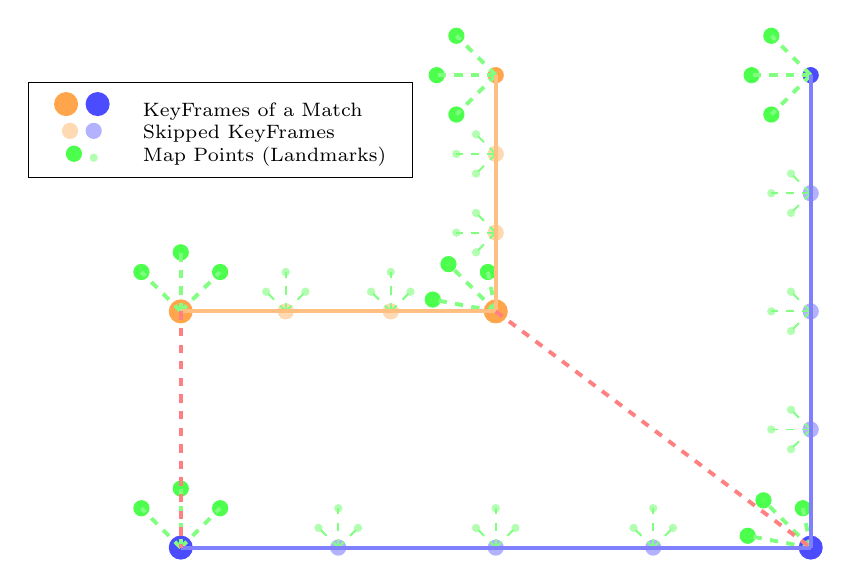
\begin{tikzpicture}
    \coordinate (A1) at (0, 3);
    \coordinate (A1MP1) at (-0.5, 3.5);
    \coordinate (A1MP2) at (0, 3.75);
    \coordinate (A1MP3) at (0.5, 3.5);

    \coordinate (AB11) at (4/3, 3);
    \coordinate (AB11MP1) at (-0.25+4/3, 3.25);
    \coordinate (AB11MP2) at (4/3, 3.5);
    \coordinate (AB11MP3) at (0.25+4/3, 3.25);

    \coordinate (AB12) at (8/3, 3);
    \coordinate (AB12MP1) at (-0.25+8/3, 3.25);
    \coordinate (AB12MP2) at (8/3, 3.5);
    \coordinate (AB12MP3) at (0.25+8/3, 3.25);

    \coordinate (B1) at (4, 3);
    \coordinate (B1MP1) at (3.2, 3.15);
    \coordinate (B1MP2) at (3.4, 3.6);
    \coordinate (B1MP3) at (3.9, 3.5);

    \coordinate (BC11) at (4, 4);
    \coordinate (BC11MP1) at (3.75, 4.25);
    \coordinate (BC11MP2) at (3.5, 4.0);
    \coordinate (BC11MP3) at (3.75, 3.75);

    \coordinate (BC12) at (4, 5);
    \coordinate (BC12MP1) at (3.75, 5.25);
    \coordinate (BC12MP2) at (3.5, 5.0);
    \coordinate (BC12MP3) at (3.75, 4.75);

    \coordinate (C1) at (4, 6);
    \coordinate (C1MP1) at (3.5, 6.5);
    \coordinate (C1MP2) at (3.25, 6.0);
    \coordinate (C1MP3) at (3.5, 5.5);

    \coordinate (A2) at (0, 0);
    \coordinate (A2MP1) at (-0.5, 0.5);
    \coordinate (A2MP2) at (0, 0.75);
    \coordinate (A2MP3) at (0.5, 0.5);

    \coordinate (AB21) at (2, 0);
    \coordinate (AB21MP1) at (1.75, 0.25);
    \coordinate (AB21MP2) at (2, 0.5);
    \coordinate (AB21MP3) at (2.25, 0.25);

    \coordinate (AB22) at (4, 0);
    \coordinate (AB22MP1) at (3.75, 0.25);
    \coordinate (AB22MP2) at (4, 0.5);
    \coordinate (AB22MP3) at (4.25, 0.25);

    \coordinate (AB23) at (6, 0);
    \coordinate (AB23MP1) at (5.75, 0.25);
    \coordinate (AB23MP2) at (6, 0.5);
    \coordinate (AB23MP3) at (6.25, 0.25);

    \coordinate (B2) at (8, 0);
    \coordinate (B2MP1) at (7.2, 0.15);
    \coordinate (B2MP2) at (7.4, 0.6);
    \coordinate (B2MP3) at (7.9, 0.5);

    \coordinate (BC21) at (8, 1.5);
    \coordinate (BC21MP1) at (7.75, 1.75);
    \coordinate (BC21MP2) at (7.5, 1.5);
    \coordinate (BC21MP3) at (7.75, 1.25);

    \coordinate (BC22) at (8, 3);
    \coordinate (BC22MP1) at (7.75, 3.25);
    \coordinate (BC22MP2) at (7.5, 3.0);
    \coordinate (BC22MP3) at (7.75, 2.75);

    \coordinate (BC23) at (8, 4.5);
    \coordinate (BC23MP1) at (7.75, 4.75);
    \coordinate (BC23MP2) at (7.5, 4.5);
    \coordinate (BC23MP3) at (7.75, 4.25);

    \coordinate (C2) at (8, 6);
    \coordinate (C2MP1) at (7.5, 6.5);
    \coordinate (C2MP2) at (7.25, 6.0);
    \coordinate (C2MP3) at (7.5, 5.5);

    \node [fill=orange!70, circle,inner sep=3pt, text width=0.1mm] at (A1) {};
    \node [fill=green!70, circle,inner sep=2pt, text width=0.1mm] at (A1MP1) {};
    \node [fill=green!70, circle,inner sep=2pt, text width=0.1mm] at (A1MP2) {};
    \node [fill=green!70, circle,inner sep=2pt, text width=0.1mm] at (A1MP3) {};
    \draw [green!50, dashed, line width=0.05cm] (A1) to (A1MP1);
    \draw [green!50, dashed, line width=0.05cm] (A1) to (A1MP2);
    \draw [green!50, dashed, line width=0.05cm] (A1) to (A1MP3);

    \node [fill=orange!30, circle,inner sep=2pt, text width=0.1mm] at (AB11) {};
    \node [fill=green!30, circle,inner sep=1pt, text width=0.1mm] at (AB11MP1) {};
    \node [fill=green!30, circle,inner sep=1pt, text width=0.1mm] at (AB11MP2) {};
    \node [fill=green!30, circle,inner sep=1pt, text width=0.1mm] at (AB11MP3) {};
    \draw [green!50, dashed, line width=0.025cm] (AB11) to (AB11MP1);
    \draw [green!50, dashed, line width=0.025cm] (AB11) to (AB11MP2);
    \draw [green!50, dashed, line width=0.025cm] (AB11) to (AB11MP3);

    \node [fill=orange!30, circle,inner sep=2pt, text width=0.1mm] at (AB12) {};
    \node [fill=green!30, circle,inner sep=1pt, text width=0.1mm] at (AB12MP1) {};
    \node [fill=green!30, circle,inner sep=1pt, text width=0.1mm] at (AB12MP2) {};
    \node [fill=green!30, circle,inner sep=1pt, text width=0.1mm] at (AB12MP3) {};
    \draw [green!50, dashed, line width=0.025cm] (AB12) to (AB12MP1);
    \draw [green!50, dashed, line width=0.025cm] (AB12) to (AB12MP2);
    \draw [green!50, dashed, line width=0.025cm] (AB12) to (AB12MP3);

    \node [fill=orange!70, circle, inner sep=3pt, text width=0.1mm] at (B1) {};
    \node [fill=green!70, circle, inner sep=2pt, text width=0.1mm] at (B1MP1) {};
    \node [fill=green!70, circle, inner sep=2pt, text width=0.1mm] at (B1MP2) {};
    \node [fill=green!70, circle, inner sep=2pt, text width=0.1mm] at (B1MP3) {};
    \draw [green!50, dashed, line width=0.05cm] (B1) to (B1MP1);
    \draw [green!50, dashed, line width=0.05cm] (B1) to (B1MP2);
    \draw [green!50, dashed, line width=0.05cm] (B1) to (B1MP3);

    \node [fill=orange!30, circle, inner sep=2pt, text width=0.1mm] at (BC11) {};
    \node [fill=green!30, circle,inner sep=1pt, text width=0.1mm] at (BC11MP1) {};
    \node [fill=green!30, circle,inner sep=1pt, text width=0.1mm] at (BC11MP2) {};
    \node [fill=green!30, circle,inner sep=1pt, text width=0.1mm] at (BC11MP3) {};
    \draw [green!50, dashed, line width=0.025cm] (BC11) to (BC11MP1);
    \draw [green!50, dashed, line width=0.025cm] (BC11) to (BC11MP2);
    \draw [green!50, dashed, line width=0.025cm] (BC11) to (BC11MP3);

    \node [fill=orange!30, circle, inner sep=2pt, text width=0.1mm] at (BC12) {};
    \node [fill=green!30, circle,inner sep=1pt, text width=0.1mm] at (BC12MP1) {};
    \node [fill=green!30, circle,inner sep=1pt, text width=0.1mm] at (BC12MP2) {};
    \node [fill=green!30, circle,inner sep=1pt, text width=0.1mm] at (BC12MP3) {};
    \draw [green!50, dashed, line width=0.025cm] (BC12) to (BC12MP1);
    \draw [green!50, dashed, line width=0.025cm] (BC12) to (BC12MP2);
    \draw [green!50, dashed, line width=0.025cm] (BC12) to (BC12MP3);

    \node [fill=orange!70, circle,inner sep=2pt, text width=0.1mm] at (C1) {};
    \node [fill=green!70, circle, inner sep=2pt, text width=0.1mm] at (C1MP1) {};
    \node [fill=green!70, circle, inner sep=2pt, text width=0.1mm] at (C1MP2) {};
    \node [fill=green!70, circle, inner sep=2pt, text width=0.1mm] at (C1MP3) {};
    \draw [green!50, dashed, line width=0.05cm] (C1) to (C1MP1);
    \draw [green!50, dashed, line width=0.05cm] (C1) to (C1MP2);
    \draw [green!50, dashed, line width=0.05cm] (C1) to (C1MP3);

    \node [fill=blue!70, circle,inner sep=3pt, text width=0.1mm] at (A2) {};
    \node [fill=green!70, circle,inner sep=2pt, text width=0.1mm] at (A2MP1) {};
    \node [fill=green!70, circle,inner sep=2pt, text width=0.1mm] at (A2MP2) {};
    \node [fill=green!70, circle,inner sep=2pt, text width=0.1mm] at (A2MP3) {};
    \draw [green!50, dashed, line width=0.05cm] (A2) to (A2MP1);
    \draw [green!50, dashed, line width=0.05cm] (A2) to (A2MP2);
    \draw [green!50, dashed, line width=0.05cm] (A2) to (A2MP3);

    \node [fill=blue!30, circle,inner sep=2pt, text width=0.1mm] at (AB21) {};
    \node [fill=green!30, circle,inner sep=1pt, text width=0.1mm] at (AB21MP1) {};
    \node [fill=green!30, circle,inner sep=1pt, text width=0.1mm] at (AB21MP2) {};
    \node [fill=green!30, circle,inner sep=1pt, text width=0.1mm] at (AB21MP3) {};
    \draw [green!50, dashed, line width=0.025cm] (AB21) to (AB21MP1);
    \draw [green!50, dashed, line width=0.025cm] (AB21) to (AB21MP2);
    \draw [green!50, dashed, line width=0.025cm] (AB21) to (AB21MP3);

    \node [fill=blue!30, circle,inner sep=2pt, text width=0.1mm] at (AB22) {};
    \node [fill=green!30, circle,inner sep=1pt, text width=0.1mm] at (AB22MP1) {};
    \node [fill=green!30, circle,inner sep=1pt, text width=0.1mm] at (AB22MP2) {};
    \node [fill=green!30, circle,inner sep=1pt, text width=0.1mm] at (AB22MP3) {};
    \draw [green!50, dashed, line width=0.025cm] (AB22) to (AB22MP1);
    \draw [green!50, dashed, line width=0.025cm] (AB22) to (AB22MP2);
    \draw [green!50, dashed, line width=0.025cm] (AB22) to (AB22MP3);

    \node [fill=blue!30, circle,inner sep=2pt, text width=0.1mm] at (AB23) {};
    \node [fill=green!30, circle,inner sep=1pt, text width=0.1mm] at (AB23MP1) {};
    \node [fill=green!30, circle,inner sep=1pt, text width=0.1mm] at (AB23MP2) {};
    \node [fill=green!30, circle,inner sep=1pt, text width=0.1mm] at (AB23MP3) {};
    \draw [green!50, dashed, line width=0.025cm] (AB23) to (AB23MP1);
    \draw [green!50, dashed, line width=0.025cm] (AB23) to (AB23MP2);
    \draw [green!50, dashed, line width=0.025cm] (AB23) to (AB23MP3);

    \node [fill=blue!70, circle,inner sep=3pt, text width=0.1mm] at (B2) {};
    \node [fill=green!70, circle,inner sep=2pt, text width=0.1mm] at (B2MP1) {};
    \node [fill=green!70, circle,inner sep=2pt, text width=0.1mm] at (B2MP2) {};
    \node [fill=green!70, circle,inner sep=2pt, text width=0.1mm] at (B2MP3) {};
    \draw [green!50, dashed, line width=0.05cm] (B2) to (B2MP1);
    \draw [green!50, dashed, line width=0.05cm] (B2) to (B2MP2);
    \draw [green!50, dashed, line width=0.05cm] (B2) to (B2MP3);

    \node [fill=blue!30, circle,inner sep=2pt, text width=0.1mm] at (BC21) {};
    \node [fill=green!30, circle,inner sep=1pt, text width=0.1mm] at (BC21MP1) {};
    \node [fill=green!30, circle,inner sep=1pt, text width=0.1mm] at (BC21MP2) {};
    \node [fill=green!30, circle,inner sep=1pt, text width=0.1mm] at (BC21MP3) {};
    \draw [green!50, dashed, line width=0.025cm] (BC21) to (BC21MP1);
    \draw [green!50, dashed, line width=0.025cm] (BC21) to (BC21MP2);
    \draw [green!50, dashed, line width=0.025cm] (BC21) to (BC21MP3);

    \node [fill=blue!30, circle,inner sep=2pt, text width=0.1mm] at (BC22) {};
    \node [fill=green!30, circle,inner sep=1pt, text width=0.1mm] at (BC22MP1) {};
    \node [fill=green!30, circle,inner sep=1pt, text width=0.1mm] at (BC22MP2) {};
    \node [fill=green!30, circle,inner sep=1pt, text width=0.1mm] at (BC22MP3) {};
    \draw [green!50, dashed, line width=0.025cm] (BC22) to (BC22MP1);
    \draw [green!50, dashed, line width=0.025cm] (BC22) to (BC22MP2);
    \draw [green!50, dashed, line width=0.025cm] (BC22) to (BC22MP3);
    
    \node [fill=blue!30, circle,inner sep=2pt, text width=0.1mm] at (BC23) {};
    \node [fill=green!30, circle,inner sep=1pt, text width=0.1mm] at (BC23MP1) {};
    \node [fill=green!30, circle,inner sep=1pt, text width=0.1mm] at (BC23MP2) {};
    \node [fill=green!30, circle,inner sep=1pt, text width=0.1mm] at (BC23MP3) {};
    \draw [green!50, dashed, line width=0.025cm] (BC23) to (BC23MP1);
    \draw [green!50, dashed, line width=0.025cm] (BC23) to (BC23MP2);
    \draw [green!50, dashed, line width=0.025cm] (BC23) to (BC23MP3);

    \node [fill=blue!70, circle,inner sep=2pt, text width=0.1mm] at (C2) {};
    \node [fill=green!70, circle, inner sep=2pt, text width=0.1mm] at (C2MP1) {};
    \node [fill=green!70, circle, inner sep=2pt, text width=0.1mm] at (C2MP2) {};
    \node [fill=green!70, circle, inner sep=2pt, text width=0.1mm] at (C2MP3) {};
    \draw [green!50, dashed, line width=0.05cm] (C2) to (C2MP1);
    \draw [green!50, dashed, line width=0.05cm] (C2) to (C2MP2);
    \draw [green!50, dashed, line width=0.05cm] (C2) to (C2MP3);

    \draw [orange!50, line width=0.05cm] (A1) to (B1);
    \draw [orange!50, line width=0.05cm] (B1) to (C1);
    \draw [blue!50, line width=0.05cm] (A2) to (B2);
    \draw [blue!50, line width=0.05cm] (B2) to (C2);

    \draw [red!50, line width=0.05cm, dashed] (A1) to (A2);
    \draw [red!50, line width=0.05cm, dashed] (B1) to (B2);

    \node[draw] at (0.5, 5.3)
    {
      \scriptsize
      \begin{tabular}{cl}
        \tikz\node[fill=orange!70, circle,inner sep=3pt, text width=0.1mm] {}; \tikz\node[fill=blue!70, circle,inner sep=3pt, text width=0.1mm] {}; & KeyFrames of a Match \\
        \tikz\node[fill=orange!30, circle,inner sep=2pt, text width=0.1mm] {}; \tikz\node[fill=blue!30, circle,inner sep=2pt, text width=0.1mm] {}; & Skipped KeyFrames \\
        \tikz\node [fill=green!70, circle, inner sep=2pt, text width=0.1mm] {}; \tikz\node[fill=green!30, circle,inner sep=1pt, text width=0.1mm] {}; & Map Points (Landmarks)
      \end{tabular}
    };
  \end{tikzpicture}%}
  \caption{Skipped five \acp{KF}}
  \label{fig:newapproach5}
\end{figure}

Then again $m$ \acp{KF} are skipped, as shown in \autoref{fig:newapproach5}, before the last \ac{KFM} was detected, shown in \autoref{fig:newapproach6}.

\begin{figure}[H]
  \centering
  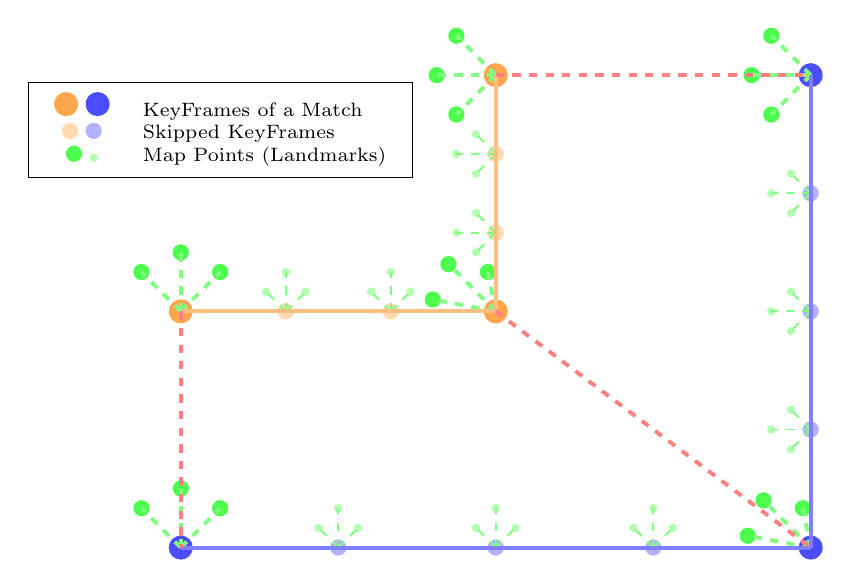
\begin{tikzpicture}
    \coordinate (A1) at (0, 3);
    \coordinate (A1MP1) at (-0.5, 3.5);
    \coordinate (A1MP2) at (0, 3.75);
    \coordinate (A1MP3) at (0.5, 3.5);

    \coordinate (AB11) at (4/3, 3);
    \coordinate (AB11MP1) at (-0.25+4/3, 3.25);
    \coordinate (AB11MP2) at (4/3, 3.5);
    \coordinate (AB11MP3) at (0.25+4/3, 3.25);

    \coordinate (AB12) at (8/3, 3);
    \coordinate (AB12MP1) at (-0.25+8/3, 3.25);
    \coordinate (AB12MP2) at (8/3, 3.5);
    \coordinate (AB12MP3) at (0.25+8/3, 3.25);

    \coordinate (B1) at (4, 3);
    \coordinate (B1MP1) at (3.2, 3.15);
    \coordinate (B1MP2) at (3.4, 3.6);
    \coordinate (B1MP3) at (3.9, 3.5);

    \coordinate (BC11) at (4, 4);
    \coordinate (BC11MP1) at (3.75, 4.25);
    \coordinate (BC11MP2) at (3.5, 4.0);
    \coordinate (BC11MP3) at (3.75, 3.75);

    \coordinate (BC12) at (4, 5);
    \coordinate (BC12MP1) at (3.75, 5.25);
    \coordinate (BC12MP2) at (3.5, 5.0);
    \coordinate (BC12MP3) at (3.75, 4.75);

    \coordinate (C1) at (4, 6);
    \coordinate (C1MP1) at (3.5, 6.5);
    \coordinate (C1MP2) at (3.25, 6.0);
    \coordinate (C1MP3) at (3.5, 5.5);

    \coordinate (A2) at (0, 0);
    \coordinate (A2MP1) at (-0.5, 0.5);
    \coordinate (A2MP2) at (0, 0.75);
    \coordinate (A2MP3) at (0.5, 0.5);

    \coordinate (AB21) at (2, 0);
    \coordinate (AB21MP1) at (1.75, 0.25);
    \coordinate (AB21MP2) at (2, 0.5);
    \coordinate (AB21MP3) at (2.25, 0.25);

    \coordinate (AB22) at (4, 0);
    \coordinate (AB22MP1) at (3.75, 0.25);
    \coordinate (AB22MP2) at (4, 0.5);
    \coordinate (AB22MP3) at (4.25, 0.25);

    \coordinate (AB23) at (6, 0);
    \coordinate (AB23MP1) at (5.75, 0.25);
    \coordinate (AB23MP2) at (6, 0.5);
    \coordinate (AB23MP3) at (6.25, 0.25);

    \coordinate (B2) at (8, 0);
    \coordinate (B2MP1) at (7.2, 0.15);
    \coordinate (B2MP2) at (7.4, 0.6);
    \coordinate (B2MP3) at (7.9, 0.5);

    \coordinate (BC21) at (8, 1.5);
    \coordinate (BC21MP1) at (7.75, 1.75);
    \coordinate (BC21MP2) at (7.5, 1.5);
    \coordinate (BC21MP3) at (7.75, 1.25);

    \coordinate (BC22) at (8, 3);
    \coordinate (BC22MP1) at (7.75, 3.25);
    \coordinate (BC22MP2) at (7.5, 3.0);
    \coordinate (BC22MP3) at (7.75, 2.75);

    \coordinate (BC23) at (8, 4.5);
    \coordinate (BC23MP1) at (7.75, 4.75);
    \coordinate (BC23MP2) at (7.5, 4.5);
    \coordinate (BC23MP3) at (7.75, 4.25);

    \coordinate (C2) at (8, 6);
    \coordinate (C2MP1) at (7.5, 6.5);
    \coordinate (C2MP2) at (7.25, 6.0);
    \coordinate (C2MP3) at (7.5, 5.5);

    \node [fill=orange!70, circle,inner sep=3pt, text width=0.1mm] at (A1) {};
    \node [fill=green!70, circle,inner sep=2pt, text width=0.1mm] at (A1MP1) {};
    \node [fill=green!70, circle,inner sep=2pt, text width=0.1mm] at (A1MP2) {};
    \node [fill=green!70, circle,inner sep=2pt, text width=0.1mm] at (A1MP3) {};
    \draw [green!50, dashed, line width=0.05cm] (A1) to (A1MP1);
    \draw [green!50, dashed, line width=0.05cm] (A1) to (A1MP2);
    \draw [green!50, dashed, line width=0.05cm] (A1) to (A1MP3);

    \node [fill=orange!30, circle,inner sep=2pt, text width=0.1mm] at (AB11) {};
    \node [fill=green!30, circle,inner sep=1pt, text width=0.1mm] at (AB11MP1) {};
    \node [fill=green!30, circle,inner sep=1pt, text width=0.1mm] at (AB11MP2) {};
    \node [fill=green!30, circle,inner sep=1pt, text width=0.1mm] at (AB11MP3) {};
    \draw [green!50, dashed, line width=0.025cm] (AB11) to (AB11MP1);
    \draw [green!50, dashed, line width=0.025cm] (AB11) to (AB11MP2);
    \draw [green!50, dashed, line width=0.025cm] (AB11) to (AB11MP3);

    \node [fill=orange!30, circle,inner sep=2pt, text width=0.1mm] at (AB12) {};
    \node [fill=green!30, circle,inner sep=1pt, text width=0.1mm] at (AB12MP1) {};
    \node [fill=green!30, circle,inner sep=1pt, text width=0.1mm] at (AB12MP2) {};
    \node [fill=green!30, circle,inner sep=1pt, text width=0.1mm] at (AB12MP3) {};
    \draw [green!50, dashed, line width=0.025cm] (AB12) to (AB12MP1);
    \draw [green!50, dashed, line width=0.025cm] (AB12) to (AB12MP2);
    \draw [green!50, dashed, line width=0.025cm] (AB12) to (AB12MP3);

    \node [fill=orange!70, circle, inner sep=3pt, text width=0.1mm] at (B1) {};
    \node [fill=green!70, circle, inner sep=2pt, text width=0.1mm] at (B1MP1) {};
    \node [fill=green!70, circle, inner sep=2pt, text width=0.1mm] at (B1MP2) {};
    \node [fill=green!70, circle, inner sep=2pt, text width=0.1mm] at (B1MP3) {};
    \draw [green!50, dashed, line width=0.05cm] (B1) to (B1MP1);
    \draw [green!50, dashed, line width=0.05cm] (B1) to (B1MP2);
    \draw [green!50, dashed, line width=0.05cm] (B1) to (B1MP3);

    \node [fill=orange!30, circle, inner sep=2pt, text width=0.1mm] at (BC11) {};
    \node [fill=green!30, circle,inner sep=1pt, text width=0.1mm] at (BC11MP1) {};
    \node [fill=green!30, circle,inner sep=1pt, text width=0.1mm] at (BC11MP2) {};
    \node [fill=green!30, circle,inner sep=1pt, text width=0.1mm] at (BC11MP3) {};
    \draw [green!50, dashed, line width=0.025cm] (BC11) to (BC11MP1);
    \draw [green!50, dashed, line width=0.025cm] (BC11) to (BC11MP2);
    \draw [green!50, dashed, line width=0.025cm] (BC11) to (BC11MP3);

    \node [fill=orange!30, circle, inner sep=2pt, text width=0.1mm] at (BC12) {};
    \node [fill=green!30, circle,inner sep=1pt, text width=0.1mm] at (BC12MP1) {};
    \node [fill=green!30, circle,inner sep=1pt, text width=0.1mm] at (BC12MP2) {};
    \node [fill=green!30, circle,inner sep=1pt, text width=0.1mm] at (BC12MP3) {};
    \draw [green!50, dashed, line width=0.025cm] (BC12) to (BC12MP1);
    \draw [green!50, dashed, line width=0.025cm] (BC12) to (BC12MP2);
    \draw [green!50, dashed, line width=0.025cm] (BC12) to (BC12MP3);

    \node [fill=orange!70, circle,inner sep=3pt, text width=0.1mm] at (C1) {};
    \node [fill=green!70, circle, inner sep=2pt, text width=0.1mm] at (C1MP1) {};
    \node [fill=green!70, circle, inner sep=2pt, text width=0.1mm] at (C1MP2) {};
    \node [fill=green!70, circle, inner sep=2pt, text width=0.1mm] at (C1MP3) {};
    \draw [green!50, dashed, line width=0.05cm] (C1) to (C1MP1);
    \draw [green!50, dashed, line width=0.05cm] (C1) to (C1MP2);
    \draw [green!50, dashed, line width=0.05cm] (C1) to (C1MP3);

    \node [fill=blue!70, circle,inner sep=3pt, text width=0.1mm] at (A2) {};
    \node [fill=green!70, circle,inner sep=2pt, text width=0.1mm] at (A2MP1) {};
    \node [fill=green!70, circle,inner sep=2pt, text width=0.1mm] at (A2MP2) {};
    \node [fill=green!70, circle,inner sep=2pt, text width=0.1mm] at (A2MP3) {};
    \draw [green!50, dashed, line width=0.05cm] (A2) to (A2MP1);
    \draw [green!50, dashed, line width=0.05cm] (A2) to (A2MP2);
    \draw [green!50, dashed, line width=0.05cm] (A2) to (A2MP3);

    \node [fill=blue!30, circle,inner sep=2pt, text width=0.1mm] at (AB21) {};
    \node [fill=green!30, circle,inner sep=1pt, text width=0.1mm] at (AB21MP1) {};
    \node [fill=green!30, circle,inner sep=1pt, text width=0.1mm] at (AB21MP2) {};
    \node [fill=green!30, circle,inner sep=1pt, text width=0.1mm] at (AB21MP3) {};
    \draw [green!50, dashed, line width=0.025cm] (AB21) to (AB21MP1);
    \draw [green!50, dashed, line width=0.025cm] (AB21) to (AB21MP2);
    \draw [green!50, dashed, line width=0.025cm] (AB21) to (AB21MP3);

    \node [fill=blue!30, circle,inner sep=2pt, text width=0.1mm] at (AB22) {};
    \node [fill=green!30, circle,inner sep=1pt, text width=0.1mm] at (AB22MP1) {};
    \node [fill=green!30, circle,inner sep=1pt, text width=0.1mm] at (AB22MP2) {};
    \node [fill=green!30, circle,inner sep=1pt, text width=0.1mm] at (AB22MP3) {};
    \draw [green!50, dashed, line width=0.025cm] (AB22) to (AB22MP1);
    \draw [green!50, dashed, line width=0.025cm] (AB22) to (AB22MP2);
    \draw [green!50, dashed, line width=0.025cm] (AB22) to (AB22MP3);

    \node [fill=blue!30, circle,inner sep=2pt, text width=0.1mm] at (AB23) {};
    \node [fill=green!30, circle,inner sep=1pt, text width=0.1mm] at (AB23MP1) {};
    \node [fill=green!30, circle,inner sep=1pt, text width=0.1mm] at (AB23MP2) {};
    \node [fill=green!30, circle,inner sep=1pt, text width=0.1mm] at (AB23MP3) {};
    \draw [green!50, dashed, line width=0.025cm] (AB23) to (AB23MP1);
    \draw [green!50, dashed, line width=0.025cm] (AB23) to (AB23MP2);
    \draw [green!50, dashed, line width=0.025cm] (AB23) to (AB23MP3);

    \node [fill=blue!70, circle,inner sep=3pt, text width=0.1mm] at (B2) {};
    \node [fill=green!70, circle,inner sep=2pt, text width=0.1mm] at (B2MP1) {};
    \node [fill=green!70, circle,inner sep=2pt, text width=0.1mm] at (B2MP2) {};
    \node [fill=green!70, circle,inner sep=2pt, text width=0.1mm] at (B2MP3) {};
    \draw [green!50, dashed, line width=0.05cm] (B2) to (B2MP1);
    \draw [green!50, dashed, line width=0.05cm] (B2) to (B2MP2);
    \draw [green!50, dashed, line width=0.05cm] (B2) to (B2MP3);

    \node [fill=blue!30, circle,inner sep=2pt, text width=0.1mm] at (BC21) {};
    \node [fill=green!30, circle,inner sep=1pt, text width=0.1mm] at (BC21MP1) {};
    \node [fill=green!30, circle,inner sep=1pt, text width=0.1mm] at (BC21MP2) {};
    \node [fill=green!30, circle,inner sep=1pt, text width=0.1mm] at (BC21MP3) {};
    \draw [green!50, dashed, line width=0.025cm] (BC21) to (BC21MP1);
    \draw [green!50, dashed, line width=0.025cm] (BC21) to (BC21MP2);
    \draw [green!50, dashed, line width=0.025cm] (BC21) to (BC21MP3);

    \node [fill=blue!30, circle,inner sep=2pt, text width=0.1mm] at (BC22) {};
    \node [fill=green!30, circle,inner sep=1pt, text width=0.1mm] at (BC22MP1) {};
    \node [fill=green!30, circle,inner sep=1pt, text width=0.1mm] at (BC22MP2) {};
    \node [fill=green!30, circle,inner sep=1pt, text width=0.1mm] at (BC22MP3) {};
    \draw [green!50, dashed, line width=0.025cm] (BC22) to (BC22MP1);
    \draw [green!50, dashed, line width=0.025cm] (BC22) to (BC22MP2);
    \draw [green!50, dashed, line width=0.025cm] (BC22) to (BC22MP3);
    
    \node [fill=blue!30, circle,inner sep=2pt, text width=0.1mm] at (BC23) {};
    \node [fill=green!30, circle,inner sep=1pt, text width=0.1mm] at (BC23MP1) {};
    \node [fill=green!30, circle,inner sep=1pt, text width=0.1mm] at (BC23MP2) {};
    \node [fill=green!30, circle,inner sep=1pt, text width=0.1mm] at (BC23MP3) {};
    \draw [green!50, dashed, line width=0.025cm] (BC23) to (BC23MP1);
    \draw [green!50, dashed, line width=0.025cm] (BC23) to (BC23MP2);
    \draw [green!50, dashed, line width=0.025cm] (BC23) to (BC23MP3);

    \node [fill=blue!70, circle,inner sep=3pt, text width=0.1mm] at (C2) {};
    \node [fill=green!70, circle, inner sep=2pt, text width=0.1mm] at (C2MP1) {};
    \node [fill=green!70, circle, inner sep=2pt, text width=0.1mm] at (C2MP2) {};
    \node [fill=green!70, circle, inner sep=2pt, text width=0.1mm] at (C2MP3) {};
    \draw [green!50, dashed, line width=0.05cm] (C2) to (C2MP1);
    \draw [green!50, dashed, line width=0.05cm] (C2) to (C2MP2);
    \draw [green!50, dashed, line width=0.05cm] (C2) to (C2MP3);

    \draw [orange!50, line width=0.05cm] (A1) to (B1);
    \draw [orange!50, line width=0.05cm] (B1) to (C1);
    \draw [blue!50, line width=0.05cm] (A2) to (B2);
    \draw [blue!50, line width=0.05cm] (B2) to (C2);

    \draw [red!50, line width=0.05cm, dashed] (A1) to (A2);
    \draw [red!50, line width=0.05cm, dashed] (B1) to (B2);
    \draw [red!50, line width=0.05cm, dashed] (C1) to (C2);

    \node[draw] at (0.5, 5.3)
    {
    \scriptsize
    \begin{tabular}{cl}
      \tikz\node[fill=orange!70, circle,inner sep=3pt, text width=0.1mm] {}; \tikz\node[fill=blue!70, circle,inner sep=3pt, text width=0.1mm] {}; & KeyFrames of a Match \\
      \tikz\node[fill=orange!30, circle,inner sep=2pt, text width=0.1mm] {}; \tikz\node[fill=blue!30, circle,inner sep=2pt, text width=0.1mm] {}; & Skipped KeyFrames \\
      \tikz\node [fill=green!70, circle, inner sep=2pt, text width=0.1mm] {}; \tikz\node[fill=green!30, circle,inner sep=1pt, text width=0.1mm] {}; & Map Points (Landmarks)
    \end{tabular}
    };
  \end{tikzpicture}
  \caption{Last \acp{KFM}}
  \label{fig:newapproach6}
\end{figure}

After the last \ac{KFM} was detected, the maps will be aligned with the transformation $T$ from the first \ac{KFM} and the \acp{MP} of the \acp{KF} belonging to a \ac{KFM} are fused, as shown in \autoref{fig:newapproach7}.

\begin{figure}[H]
  \centering
  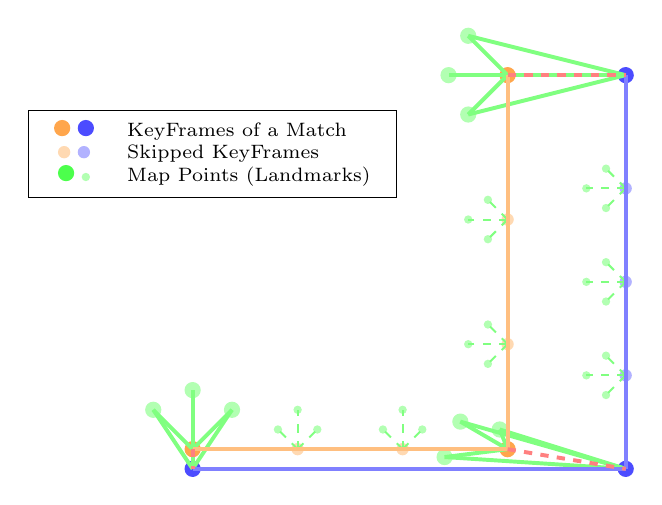
\begin{tikzpicture}
    \coordinate (A1) at (0, 0.25);
    \coordinate (A1MP1) at (-0.5, 0.75);
    \coordinate (A1MP2) at (0, 1.0);
    \coordinate (A1MP3) at (0.5, 0.75);

    \coordinate (AB11) at (4/3, 0.25);
    \coordinate (AB11MP1) at (-0.25+4/3, 0.5);
    \coordinate (AB11MP2) at (4/3, 0.75);
    \coordinate (AB11MP3) at (0.25+4/3, 0.5);

    \coordinate (AB12) at (8/3, 0.25);
    \coordinate (AB12MP1) at (-0.25+8/3, 0.5);
    \coordinate (AB12MP2) at (8/3, 0.75);
    \coordinate (AB12MP3) at (0.25+8/3, 0.5);

    \coordinate (B1) at (4, 0.25);
    \coordinate (B1MP1) at (3.2, 0.15);
    \coordinate (B1MP2) at (3.4, 0.6);
    \coordinate (B1MP3) at (3.9, 0.5);

    \coordinate (BC11) at (4, 4.75/3);
    \coordinate (BC11MP1) at (3.75, 4.75/3 + 0.25);
    \coordinate (BC11MP2) at (3.5, 4.75/3);
    \coordinate (BC11MP3) at (3.75, 4.75/3 - 0.25);

    \coordinate (BC12) at (4, 4.75/1.5);
    \coordinate (BC12MP1) at (3.75, 4.75/1.5 + 0.25);
    \coordinate (BC12MP2) at (3.5, 4.75/1.5);
    \coordinate (BC12MP3) at (3.75, 4.75/1.5 - 0.25);

    \coordinate (C1) at (4, 5);
    \coordinate (C1MP1) at (3.5, 5.5);
    \coordinate (C1MP2) at (3.25, 5.0);
    \coordinate (C1MP3) at (3.5, 4.5);

    \coordinate (A2) at (0, 0);

    \coordinate (B2) at (5.5, 0);

    \coordinate (BC21) at (5.5, 4.75/4);
    \coordinate (BC21MP1) at (5.25, 4.75/4 + 0.25);
    \coordinate (BC21MP2) at (5.0, 4.75/4);
    \coordinate (BC21MP3) at (5.25, 4.75/4 - 0.25);

    \coordinate (BC22) at (5.5, 4.75/2);
    \coordinate (BC22MP1) at (5.25, 4.75/2 + 0.25);
    \coordinate (BC22MP2) at (5.0, 4.75/2);
    \coordinate (BC22MP3) at (5.25, 4.75/2 - 0.25);

    \coordinate (BC23) at (5.5, 3*4.75/4);
    \coordinate (BC23MP1) at (5.25, 3*4.75/4 + 0.25);
    \coordinate (BC23MP2) at (5.0, 3*4.75/4);
    \coordinate (BC23MP3) at (5.25, 3*4.75/4 - 0.25);

    \coordinate (C12) at (4.5, 5.0);
    \coordinate (C2) at (5.5, 5);

    \node [fill=orange!70, circle,inner sep=2pt, text width=0.1mm] at (A1) {};
    \node [fill=green!30, circle,inner sep=2pt, text width=0.1mm] at (A1MP1) {};
    \node [fill=green!30, circle,inner sep=2pt, text width=0.1mm] at (A1MP2) {};
    \node [fill=green!30, circle,inner sep=2pt, text width=0.1mm] at (A1MP3) {};
    \draw [green!50, line width=0.05cm] (A1) to (A1MP1);
    \draw [green!50, line width=0.05cm] (A1) to (A1MP2);
    \draw [green!50, line width=0.05cm] (A1) to (A1MP3);

    \node [fill=orange!30, circle,inner sep=1.5pt, text width=0.1mm] at (AB11) {};
    \node [fill=green!30, circle,inner sep=1pt, text width=0.1mm] at (AB11MP1) {};
    \node [fill=green!30, circle,inner sep=1pt, text width=0.1mm] at (AB11MP2) {};
    \node [fill=green!30, circle,inner sep=1pt, text width=0.1mm] at (AB11MP3) {};
    \draw [green!50, dashed, line width=0.025cm] (AB11) to (AB11MP1);
    \draw [green!50, dashed, line width=0.025cm] (AB11) to (AB11MP2);
    \draw [green!50, dashed, line width=0.025cm] (AB11) to (AB11MP3);

    \node [fill=orange!30, circle,inner sep=1.5pt, text width=0.1mm] at (AB12) {};
    \node [fill=green!30, circle,inner sep=1pt, text width=0.1mm] at (AB12MP1) {};
    \node [fill=green!30, circle,inner sep=1pt, text width=0.1mm] at (AB12MP2) {};
    \node [fill=green!30, circle,inner sep=1pt, text width=0.1mm] at (AB12MP3) {};
    \draw [green!50, dashed, line width=0.025cm] (AB12) to (AB12MP1);
    \draw [green!50, dashed, line width=0.025cm] (AB12) to (AB12MP2);
    \draw [green!50, dashed, line width=0.025cm] (AB12) to (AB12MP3);

    \node [fill=orange!70, circle,inner sep=2pt, text width=0.1mm] at (B1) {};
    \node [fill=green!30, circle, inner sep=2pt, text width=0.1mm] at (B1MP1) {};
    \node [fill=green!30, circle, inner sep=2pt, text width=0.1mm] at (B1MP2) {};
    \node [fill=green!30, circle, inner sep=2pt, text width=0.1mm] at (B1MP3) {};
    \draw [green!50, line width=0.05cm] (B1) to (B1MP1);
    \draw [green!50, line width=0.05cm] (B1) to (B1MP2);
    \draw [green!50, line width=0.05cm] (B1) to (B1MP3);

    \node [fill=orange!30, circle, inner sep=1.5pt, text width=0.1mm] at (BC11) {};
    \node [fill=green!30, circle,inner sep=1pt, text width=0.1mm] at (BC11MP1) {};
    \node [fill=green!30, circle,inner sep=1pt, text width=0.1mm] at (BC11MP2) {};
    \node [fill=green!30, circle,inner sep=1pt, text width=0.1mm] at (BC11MP3) {};
    \draw [green!50, dashed, line width=0.025cm] (BC11) to (BC11MP1);
    \draw [green!50, dashed, line width=0.025cm] (BC11) to (BC11MP2);
    \draw [green!50, dashed, line width=0.025cm] (BC11) to (BC11MP3);

    \node [fill=orange!30, circle, inner sep=1.5pt, text width=0.1mm] at (BC12) {};
    \node [fill=green!30, circle,inner sep=1pt, text width=0.1mm] at (BC12MP1) {};
    \node [fill=green!30, circle,inner sep=1pt, text width=0.1mm] at (BC12MP2) {};
    \node [fill=green!30, circle,inner sep=1pt, text width=0.1mm] at (BC12MP3) {};
    \draw [green!50, dashed, line width=0.025cm] (BC12) to (BC12MP1);
    \draw [green!50, dashed, line width=0.025cm] (BC12) to (BC12MP2);
    \draw [green!50, dashed, line width=0.025cm] (BC12) to (BC12MP3);

    \node [fill=orange!70, circle,inner sep=2pt, text width=0.1mm] at (C1) {};
    \node [fill=green!30, circle, inner sep=2pt, text width=0.1mm] at (C1MP1) {};
    \node [fill=green!30, circle, inner sep=2pt, text width=0.1mm] at (C1MP2) {};
    \node [fill=green!30, circle, inner sep=2pt, text width=0.1mm] at (C1MP3) {};
    \draw [green!50, line width=0.05cm] (C1) to (C1MP1);
    \draw [green!50, line width=0.05cm] (C1) to (C1MP2);
    \draw [green!50, line width=0.05cm] (C1) to (C1MP3);

    \node [fill=blue!70, circle,inner sep=2pt, text width=0.1mm] at (A2) {};
    \draw [green!50, line width=0.05cm] (A2) to (A1MP1);
    \draw [green!50, line width=0.05cm] (A2) to (A1MP2);
    \draw [green!50, line width=0.05cm] (A2) to (A1MP3);

    \node [fill=blue!70, circle,inner sep=2pt, text width=0.1mm] at (B2) {};
    \draw [green!50, line width=0.05cm] (B2) to (B1MP1);
    \draw [green!50, line width=0.05cm] (B2) to (B1MP2);
    \draw [green!50, line width=0.05cm] (B2) to (B1MP3);

    \node [fill=blue!30, circle,inner sep=1.5pt, text width=0.1mm] at (BC21) {};
    \node [fill=green!30, circle,inner sep=1pt, text width=0.1mm] at (BC21MP1) {};
    \node [fill=green!30, circle,inner sep=1pt, text width=0.1mm] at (BC21MP2) {};
    \node [fill=green!30, circle,inner sep=1pt, text width=0.1mm] at (BC21MP3) {};
    \draw [green!50, dashed, line width=0.025cm] (BC21) to (BC21MP1);
    \draw [green!50, dashed, line width=0.025cm] (BC21) to (BC21MP2);
    \draw [green!50, dashed, line width=0.025cm] (BC21) to (BC21MP3);

    \node [fill=blue!30, circle,inner sep=1.5pt, text width=0.1mm] at (BC22) {};
    \node [fill=green!30, circle,inner sep=1pt, text width=0.1mm] at (BC22MP1) {};
    \node [fill=green!30, circle,inner sep=1pt, text width=0.1mm] at (BC22MP2) {};
    \node [fill=green!30, circle,inner sep=1pt, text width=0.1mm] at (BC22MP3) {};
    \draw [green!50, dashed, line width=0.025cm] (BC22) to (BC22MP1);
    \draw [green!50, dashed, line width=0.025cm] (BC22) to (BC22MP2);
    \draw [green!50, dashed, line width=0.025cm] (BC22) to (BC22MP3);

    \node [fill=blue!30, circle,inner sep=1.5pt, text width=0.1mm] at (BC23) {};
    \node [fill=green!30, circle,inner sep=1pt, text width=0.1mm] at (BC23MP1) {};
    \node [fill=green!30, circle,inner sep=1pt, text width=0.1mm] at (BC23MP2) {};
    \node [fill=green!30, circle,inner sep=1pt, text width=0.1mm] at (BC23MP3) {};
    \draw [green!50, dashed, line width=0.025cm] (BC23) to (BC23MP1);
    \draw [green!50, dashed, line width=0.025cm] (BC23) to (BC23MP2);
    \draw [green!50, dashed, line width=0.025cm] (BC23) to (BC23MP3);

    \node [fill=blue!70, circle,inner sep=2pt, text width=0.1mm] at (C2) {};
    \draw [green!50, line width=0.05cm] (C2) to (C1MP1);
    \draw [green!50, line width=0.05cm] (C2) to (C1MP2);
    \draw [green!50, line width=0.05cm] (C2) to (C1MP3);

    \draw [orange!50, line width=0.05cm] (A1) to (B1);
    \draw [orange!50, line width=0.05cm] (B1) to (C1);
    \draw [blue!50, line width=0.05cm] (A2) to (B2);
    \draw [blue!50, line width=0.05cm] (B2) to (C2);

    \draw [red!50, line width=0.05cm, dashed] (A1) to (A2);
    \draw [red!50, line width=0.05cm, dashed] (B1) to (B2);
    \draw [red!50, line width=0.05cm, dashed] (C1) to (C2);

    \node[draw] at (0.25, 4.0)
    {
      \scriptsize
      \begin{tabular}{cl}
        \tikz\node[fill=orange!70, circle,inner sep=2pt, text width=0.1mm] {}; \tikz\node[fill=blue!70, circle,inner sep=2pt, text width=0.1mm] {}; & KeyFrames of a Match \\
        \tikz\node[fill=orange!30, circle,inner sep=1.5pt, text width=0.1mm] {}; \tikz\node[fill=blue!30, circle,inner sep=1.5pt, text width=0.1mm] {}; & Skipped KeyFrames \\
        \tikz\node [fill=green!70, circle, inner sep=2pt, text width=0.1mm] {}; \tikz\node[fill=green!30, circle,inner sep=1pt, text width=0.1mm] {}; & Map Points (Landmarks)
      \end{tabular}
    };
  \end{tikzpicture}%}
  \caption{Maps aligned}
  \label{fig:newapproach7}
\end{figure}

After the two maps are aligned (possibly with still some miss alignment as in \autoref{fig:newapproach7}) the \ac{PGO} can be performed which optimizes the poses of the \acp{KF} and afterwards the \ac{BA} will be performed which optimizes the poses of both, the \acp{KF} and the \acp{MP}.\\

The idea behind the usage of multiple \acp{KFM} was already discussed in contrary to the idea of skipping \acp{KF} after a \ac{KFM} was detected. This idea will be discussed next.

If \acp{KF} are skipped after \ac{KFM} was detected, the next \ac{KFM} will potentially have a bigger distance to the previous \ac{KFM}. This causes that the \acp{KFM} will be more apart from each other and therefor they will cover a bigger area. The \acp{KFM} from a bigger area provide the \ac{PGO} and the \ac{BA} with more information which hopefully leads to a reduction in drift and an increased accuracy.
\textcolor{red}{\textbf{!!!Check \ac{PGO} implementation!!!}}

To visualize the influence of this idea, \autoref{fig:kfskip1} shows the co-visibility graph of an experiment where only one \ac{KF} was skipped after a \ac{KFM} was detected. \autoref{fig:kfskip2} on the other hand shows an experiment where 10 \acp{KF} were skipped after a \ac{KFM} was detected. One can easily see, that the \acp{KFM} in \autoref{fig:kfskip2} are more apart from each other and cover a bigger area compared to the \acp{KFM} in \autoref{fig:kfskip1}.

\begin{figure}[H]
   \centering
   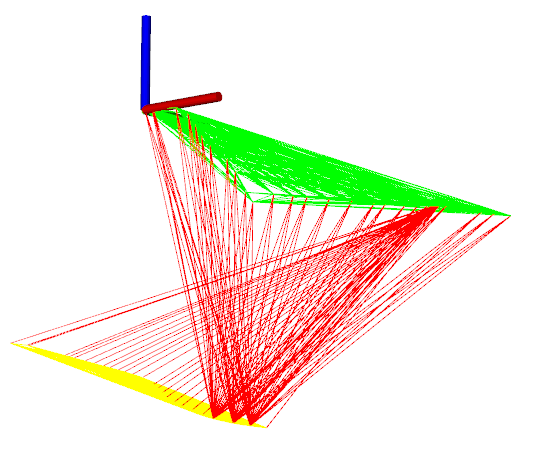
\includegraphics[width=0.75\textwidth]{images/covgraph_minHits_5_skip_1}
   \caption{1 \ac{KF} skipped after a \ac{KFM} was found\\
   \textcolor{green}{green}: Co-visibility graph of first map\\ \textcolor{yellow}{yellow}: Co-visibility graph of second map\\ \textcolor{red}{red}: Co-visibility between the \acp{KFM}}
   \label{fig:kfskip1}
\end{figure}

\begin{figure}[H]
   \centering
   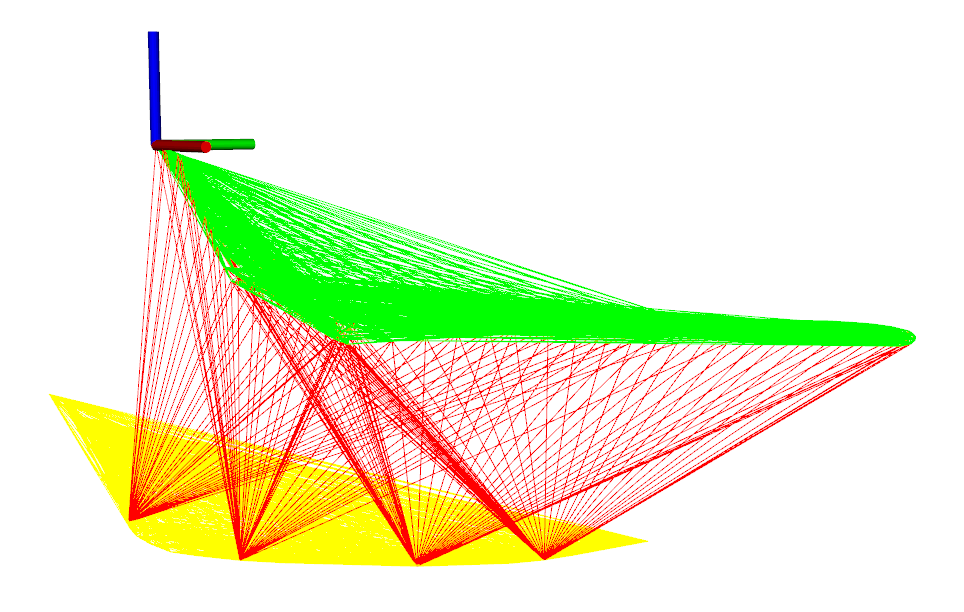
\includegraphics[width=0.75\textwidth]{images/covgraph_minHits_5_skip_10}
   \caption{10 \acp{KF} skipped after a \ac{KFM} was found\\
   \textcolor{green}{green}: Co-visibility graph of first map\\ \textcolor{yellow}{yellow}: Co-visibility graph of second map\\ \textcolor{red}{red}: Co-visibility between the \acp{KFM}}
   \label{fig:kfskip2}
\end{figure}
